\chapter{Introduction}
\label{chapter:introduction}

%\minitoc
%\chapterwithfigures{\nameref*{chapter:introduction}}
%\chapterwithtables{\nameref*{chapter:introduction}}

\ifthenelse{\boolean{skipIntro}}{\endinput}{}

\emph{Perspicere} - \textit{to see through}. Behind the Perspective's etymology is hidden the notion of portraying our three-dimensional physical reality onto a two-dimensional plane. Such concept has been extensively studied for centuries, and found its oldest fundation in the geometry Euclide defined in his \textbf{Elements} (300BC). Florence, with its artists and architects, paved the way during Quattrocento in Italian Renaissance of linear perspective studies, to represent as accurately as possible surrounding world on paintings and drawings. Brunelleschi (1377-1446) is one the very first that studied how lines, shapes, objects change under different viewpoint observation, at changing angles. Defined with lines of sights that should converge on one or several vanishing points, linear perspective aims to simulate world objects appearance as a viewer's eye would see them.

\begin{figure}[h!]
      \begin{center}
      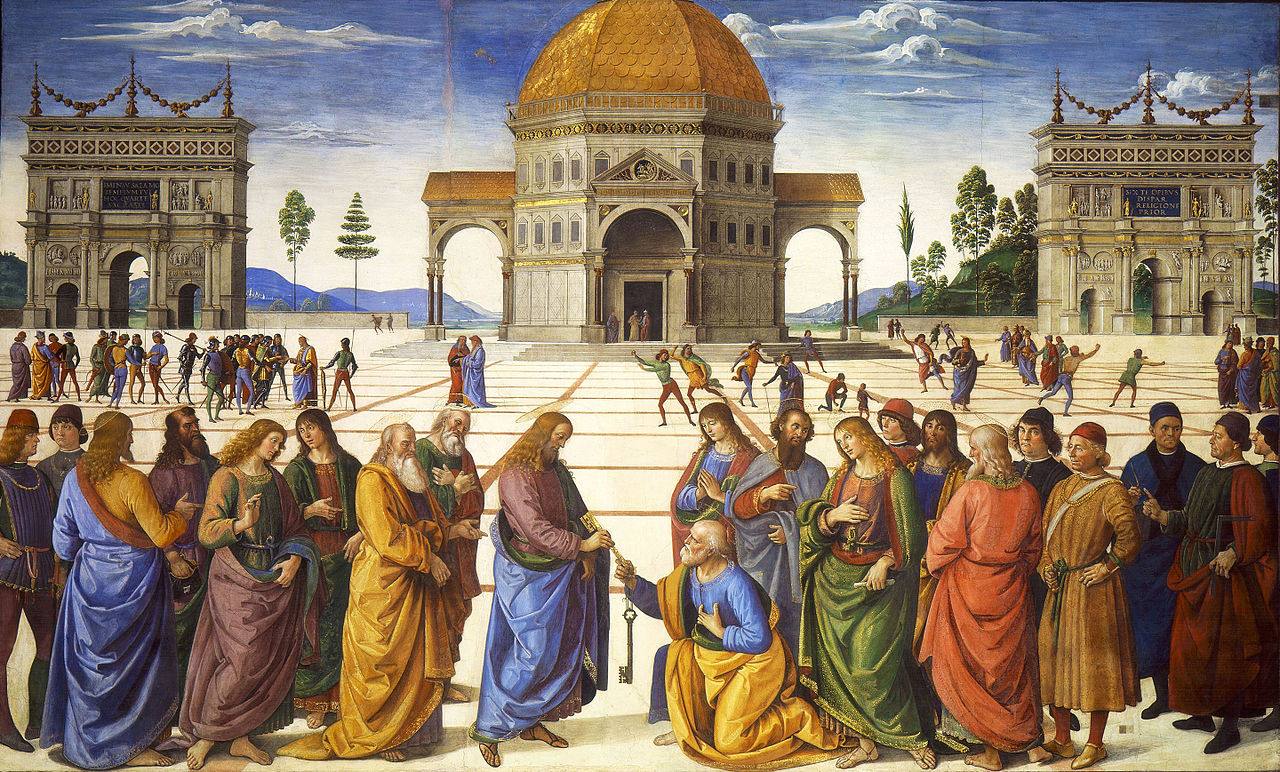
\includegraphics[width=.8\textwidth]{images/introduction/perugino.jpg}
      \end{center}
      \caption{\textit{The Delivery of the Keys}, 1481–1482, Sistine Chapel, Rome by Perugino (1481–1482). This impressive $3.3m \times 5.5m$ fresco that both illustrated linear perspective and Brunelleschi's architectural style.}
      \label{fig:intro_perugino}
\end{figure}

Even through artistic perspective studies were extremely well-tuned from a technical and mechanical standpoint \citep{simon2021jan}, perspective found new expressions in sciences few centuries later, through the advent of photogrammetry. Notion speaks for itself when we once again at its grec ethymology, \textit{photo} - \ie light -, \textit{gramma} - \ie drawing, writing - and \textit{metron} - \ie measure -. Aimé Laussedat, a French astronomer, geodesist, surveyor and cartographer used the \textit{Hôtel des Invalides} in 1849 to observe, measure and thus try to reproduce physical spaces, lines and objects from multiples perspective views. Photogrammetry therefore leverages parallax effect to extract depth and dimensions from our physical world with observed views and was intensively used during mid last century for military purposes. The advent of aerial photography, enabled by recent advancements in aviation, allowed for the topographic mapping of entire countries during the Interwar period.

\begin{figure}[h!]
      \begin{center}
      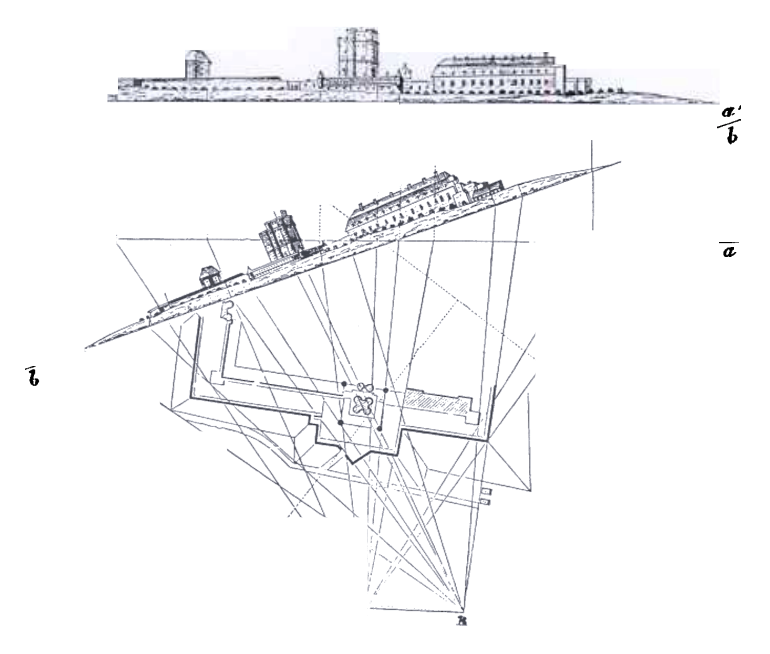
\includegraphics[width=.5\textwidth]{images/introduction/laussedat_phtograpmetrie.png}
      \end{center}
      \caption{Surveyed by the method of graphical intersections applied to perspectives recorded with the camera lucida. Survey of the Château de Vincennes by A. Laussedat, 1850}
      \label{fig:intro_laussedat}
\end{figure}

Photogrammetry has finally been heavily studied through the prism of robotics and computer vision during 1980's, with increasing computational power and emerging digital imaging technology. Structure-from-Motion approaches naturally arised from such an increasingly strong convergence between photogrammetry and computer vision in the meantime, via pioneered work from Shimon Ullman \citep{ullman1979interpretation}. Such a domain paved the way on novel view synthesis issues (and 3D reconstruction) by filling the gap between photographic scenes capturing processes and their comprehensive three-dimensional representation. 

\ac{AI}, in its commonly broad, unclear, and somewhat disputed definition within society, has a suprisingly more than a 70 years background history, with Alan Turning as the most ackwolegded earliest founding fathers of computer science \citep{turing1950computing} and artificial intelligence with John McCarthy. \ac{AI} is defined by \href{https://www.britannica.com/technology/artificial-intelligence}{The Encyclopedia Britannica} as \textit{"the ability of a computer to perform tasks commonly associated with intelligent beings"}. In the realm of Computer Vision and Graphics, this manuscript frames in a shrinked domain of \ac{AI}, commonly refered as \ac{DL}: \ac{DNN} are thus going to be considered in a large extend in the next few pages... 

\ac{DL} has itself a pationate and outstanding past history, whose one of most recognizable figures today in vision community is Yann LeCun. He has now been working over the last 30 years on vision \ac{AI} considerations, and notably introduced \ac{CNN} \citep{lecun1998gradient}, that have been widely used over the last three years of this thesis. The release in 2009 of ImageNet \citep{deng2009imagenet}, a million annotated images database, and the \ac{CNN} based image-classifier AlexNet \citep{krizhevsky2012imagenet} in 2012 are unanimously seen as the \ac{DL} breaktrhought debut. Vision tasks that were tackled by such \ac{DL} algorithms quickly grows in complexity, from segmentation \citep{long2015fully} to detection \citep{girshick2015fast} or image generation model \ac{GAN} \citep{goodfellow2014generative}. Whereas vision 2D image-based issues have thus seen substantial gains over the last decade, third dimension to adress 3D issues from our surrounding world has been added and considered since only few years, driven by latest \ac{GPU} computing advances. Through 3D geometrical prior integration considerations for novel view synthesis, this thesis thereby finds its place within the premises of what 3D AI, on the verge of a major growth in the forthcoming years, represents today.  


\section{PhD Context}

\subsection{Meero}
Meero is a Software-as-a-Service french startup founded in 2014 that primarily aims to provide \ac{AI}-powered visual enhancement tools and algorithms for businesses across several verticals, from real estate agencies to e-commerce and fashion industries, as well as automotive car dealerships. Meero proposes a wide range of \ac{AI}-based solutions, from sky replacement, virtual staging or object eraser algorithms for the real-estate vertical to background removal or virtual try-on for fashion and e-commerce companies. Regarding its automotive branch, brand as \textit{CarCutter}, Meero offers car dealerships and marketplaces the opportunity to have visually coherent and appealing images. One of its latest product refers as the 360\degree spin, that allow to virtually smoothly turn around a car given a limited set of images. Such a 3D-based application is inherantly covered by \ac{NVS} as soon as unseen viewpoint must be rendered. 

However, fundamental research in computer vision and its conterpart application in industries suffers from a massive gap that needs to be closed: most of academic papers in vision research deal with images that roughly size from $128\times128$ to $1024\times1024$, whereas images from any mobile device now have at least a 2K resolution (up to 4 to 6K for the latest DSLR camera). Even through such claim tends to thin out with latest fundation models and exploding \ac{GPU} compute capabilities, such an image resolution discrepancy prevent, during this thesis, to directly build an image-based \ac{AI} product in industy from an academic vision paper. This thesis somehow tried to filled this gap, mostly by investigating generalizable single-image novel view synthesis architecture, that could thus be non-restricted to a single scene. 

\subsection{3D reconstruction}
 \ac{NVS} is somehow inherently intertwined with 3D reconstruction, as synthesis of novel views was historically de facto allowed once the complete 3D representation was acquired. While an impressive variety of approaches exists for addressing this issue; from photogrammetry-based or Structure-From-X techniques (where X could stands for \textit{Texture, Shading, Silhouette} etc) to structured-lights ones, pionner work in such area get considerations for stereo vision \citep{marr1976cooperative} via an iterative cooperative algorithm between two views. 
 
 First \ac{AI}-based 3D reconstruction algorithms started to emerge from 2018 with seminal research from \citep{kato2018neural} that introduces one of the first differentiable neural renderer. PyTorch3D \citep{ravi2020pytorch3d} releases for  \ac{DL}-based 3D code development has played a significant role in the widespread adoption of 3D issues among the scientific community. From multi-view \citep{li2023neuralangelo} to even single-image \citep{voleti2024sv3d} 3D reconstruction, latest groundbreaking advances in 2023/2024 herald an exciting future for research in this field. 

\subsection{Novel View Synthesis}
\ac{NVS} presents a challenging task in computer vision, wherein the objective is to generate an image from an unobserved viewpoint using only a limited number of source images and their corresponding camera pose information. This thesis is almost exclusively focused toward the more intricate scenario, which exclusively relies on a unique source image. In 1998, Thomas Vetter presented a stunning approach \cite{vetter1998synthesis} for single face image \ac{NVS}, where views were used to \textit{learn} pose-invariant descriptors and by leveraging a single 3D human head generic model. \ac{NVS} has naturally started being considered through \ac{AI} prism in 2015 \citep{yang2015weakly}, even though camera displacement were discretized, preventing novel view rendering from any free viewpoint. The branch masively benefited in late 2020 from a simple, yet outstandingly powerful, novel framework concept, referred as \ac{NeRF} \cite{mildenhall2020nerf}. Few months ago, \ac{GS} models had once again disrupted the field, allowing novel view synthesis in realtime with 2K resolution images with consumer \ac{GPU} machines. 


\section{Contributions}
Aiming to perform novel viewpoint synthesis from a single-image is an extremely ill posed-problem since too many details, structures or texture are unobserved on the provided source view. Core problem that thus inherantly rises from the later observation is to find ways, such as efficient pose encoding, structural constraints that bring as many as possible prior information to the \ac{NN}. 

Years before 2023 emergence of \ac{GenAI} and incredibly powerful foundation models \citep{awais2023foundational}, dataset images we dealt with in single-image \ac{NVS} were mostly low resolution, size $128\times128$, as in ShapeNet \citep{ShapeNet}. We tried through this thesis to incorporate, as much as we possibly could, epipolar geometrical constraints and concepts. We were convinced by the same guiding principle for the last three years: \textit{the most fundamental 3D geometric considerations such as epipolar geometry must be explicitly integrated into deep neural networks.}

We tackle the \ac{NVS} problem with several approaches during this thesis, that could be summarized as follow.
\begin{itemize}
      \item \autoref{chapter:epipolarnvs}: \nameref{chapter:epipolarnvs}\\
            We start approaching single-image \ac{NVS} through the prism of camera transformation encoding. Such an information is vital for any \ac{NN} that performs \ac{NVS}, and its integration as a apriori information is far from being trivial. While several approaches exist to feed such intrinsic and extrinsic parameters to a network, we present in this chapter a novel method to encode such a camera transformation, by extensively leveraging on epipolar geometry. The work in this chapter has led to the following conference publication:
            \begin{itemize}
                \item \fullcite{landreau2022epipolarnvs}
            \end{itemize}


      \item \autoref{chapter:epinerf}: \nameref{chapter:epinerf}\\
            We then turn from camera pose encoding to inner 3D constraints consideration in \ac{NeRF}. However, we maintain the epipolar geometry concept in our work and build a feature-based attention mechanism thanks to \ac{NeRF}-based additional network, called \textit{NeRFeature}. Such a mecanism is direclty involved at training time, while we \textit{do not} have access to the target view to build epipolar constraints. Our work is currently in submission:
            \begin{itemize}
                  \item \fullcite{landreau2024epinerf}
            \end{itemize}

      \item \autoref{chapter:gausssplat}: \nameref{chapter:gausssplat}\\
            We finally relaxed the main hypothesis we dealt with in these first two apparoches to work with \ac{NVS} in a multiple-images scenario with 3D \ac{GS}. Such work mostly rely on \textit{CarCutter} 
industrial considerations, as the next generation of the current 360\degree spin stabilization. However, if rendering at training locations goes fine, stabilizing camera path to render unobserved viewpoint, and thus create seamless 360\degree car animation. 
\end{itemize}
